\usepackage{adjustbox}
\usepackage{adjustbox}
  author={Ngo, Hien Quoc and Ashikhmin, Alexei and Yang, Hong and Larsson, Erik G and Marzetta, Thomas L},

@article{ngo2017cell,
\begin{filecontents*}{refs.bib}
@article{ngo2017cell,
  title={Cell-free massive MIMO versus small cells},
\usepackage{float}
  author={Ngo, Hien Quoc and Ashikhmin, Alexei and Yang, Hong and Larsson, Erik G and Marzetta, Thomas L},
  journal={IEEE Transactions on Wireless Communications},
  author={Demir, Ozgecan and Bj\"ornson, Emil and Sanguinetti, Luca},
  volume={16},
  number={3},
  pages={1834--1850},
  year={2017}
}

@article{demir2021foundations,
  author={Buzzi, Stefano and D'Andrea, Carmen},

  title={Foundations of Cell-Free Massive MIMO},
  author={Demir, Ozgecan and Bj\"ornson, Emil and Sanguinetti, Luca},
  journal={Foundations and Trends in Signal Processing},
  volume={14},
  number={3--4},
  pages={162--472},
  author={Nayebi, Elina and Ashikhmin, Alexei and Marzetta, Thomas L and Yang, Hong},
  year={2021}
}

@article{buzzi2019user,

  pages={3594--3608},
  title={User-centric cell-free massive MIMO: A new approach to wireless communication},
  author={Bashar, Moinul and Cumanan, Kanapathippillai and Burr, Alister G and Ngo, Hien Quoc and Larsson, Erik G},
  author={Buzzi, Stefano and D'Andrea, Carmen},
  journal={IEEE Wireless Communications Letters},
  volume={9},
  number={1},
  pages={83--87},
  year={2019}
}
  author={Bj\"ornson, Emil and Sanguinetti, Luca},

@article{nayebi2017precoding,
  title={Precoding and power optimization in cell-free massive MIMO systems},

  author={Nayebi, Elina and Ashikhmin, Alexei and Marzetta, Thomas L and Yang, Hong},
  journal={IEEE Transactions on Wireless Communications},

  author={Interdonato, Giovanni and Karlsson, Martin and Bj{\"o}rnson, Emil and Larsson, Erik G},
  volume={16},
The literature on cell-free massive MIMO has expanded significantly, focusing on user association strategies and the integration of advanced computational models like QUBO and Ising machines. Previous studies such as \cite{bashar2019uplink, chen2018channel, zhang2021improving} have explored various aspects of this technology, providing a foundation for further exploration.

Physics-inspired optimization has gained traction for scheduling, resource allocation, and user association \cite{kasi2021resource,grassl2022ising}. Coherent Ising machines and annealers aim to find low-energy states of Ising Hamiltonians, to which many combinatorial problems can be mapped via QUBO \cite{lucas2014ising,mcmahon2016fully,inagaki2016coherent,glover2018tutorial}. Applications to wireless include link scheduling, channel assignment, and preliminary cell-free formulations \cite{zhao2022joint}. Compared to prior work, our contribution offers: (i) a first-principles interference-aware QUBO with pairwise terms derived from MRT projections, (ii) a fairness-weighted QUBO variant for proportional-fair behavior, and (iii) a complete two-level flow with feasibility projection, strong baselines, statistical rigor, and discussion of hardware mapping and scalability.

Our work is distinct in its comprehensive approach to integrating QUBO with cell-free massive MIMO systems. We extend beyond existing literature by providing a detailed methodology for AP selection and precoding, leveraging Ising-style solvers for efficient combinatorial optimization.

\begin{abstract}
  number={7},
  pages={4445--4459},
  year={2017}
}

  author={Chen, Shanzhi and Zhang, Jun and Ai, Bo and Bj{\"o}rnson, Emil and Zhong, Zhangdui},
@article{bashar2019uplink,
  title={Uplink performance of cell-free massive MIMO with multi-antenna users},
  author={Bashar, Moinul and Cumanan, Kanapathippillai and Burr, Alister G and Ngo, Hien Quoc and Larsson, Erik G},
  journal={IEEE Transactions on Wireless Communications},
  volume={18},
  number={7},
  pages={3594--3608},
Large language models have demonstrated remarkable capabilities in various domains, including natural language understanding, generation, and reasoning tasks. Recent advances have particularly focused on improving their reliability and factual accuracy through various prompting and fine-tuning strategies.
  author={Zhang, Jian and Chen, Shanzhi and Bj{\"o}rnson, Emil and Debbah, M{\'e}rouane and Ai, Bo},
  year={2019}
}

@article{bjornson2019making,
  title={Making cell-free massive MIMO competitive with MMSE processing and centralized implementation},
  author={Bj\"ornson, Emil and Sanguinetti, Luca},
  journal={IEEE Transactions on Wireless Communications},
  author={Bj{\"o}rnson, Emil and Van der Perre, Liesbet and Buzzi, Stefano and Larsson, Erik G},
  volume={19},
  number={1},
  pages={77--90},
  year={2020}

The literature on cell-free massive MIMO has expanded significantly, focusing on user association strategies and the integration of advanced computational models like QUBO and Ising machines. Previous studies such as \cite{bashar2019uplink, chen2018channel, zhang2021improving} have explored various aspects of this technology, providing a foundation for further exploration.


}

  author={Peel, C. B. and Hochwald, B. M. and Swindlehurst, A. L.},
@article{interdonato2019scalability,
  title={Scalability aspects of cell-free massive MIMO},
  author={Interdonato, Giovanni and Karlsson, Martin and Bj{\"o}rnson, Emil and Larsson, Erik G},
  journal={IEEE Wireless Communications Letters},
  volume={8},
  number={6},
  pages={1689--1693},
  author={Lucas, Andrew},
  year={2019}
}

@article{chen2020structured,
  title={Structured user-centric cell-free massive MIMO: A new approach to scalable and energy-efficient wireless networks},
In this paper, we propose a novel approach to address these challenges using a two-level framework involving Quadratic Unconstrained Binary Optimization (QUBO) and a Coherent Ising Machine (CIM).
  author={Chen, Shanzhi and Zhang, Jun and Ai, Bo and Bj{\"o}rnson, Emil and Zhong, Zhangdui},
  author={Glover, Fred and Kochenberger, Gary and Du, Yu},
  journal={IEEE Wireless Communications},
  volume={28},
  number={1},
  pages={220--226},
  year={2021}
}

  author={McMahon, Peter L. and Marandi, Alireza and Haribara, Yoshihisa and Hamerly, Ryan and Langrock, Carsten and Tamate, Shuhei and Inagaki, Takahiro and Takesue, Hiroki and Utsunomiya, Shoko and Aihara, Kazuyuki and others},
@article{zhang2019cell,
  title={Cell-free massive MIMO: A new look at interference},
  author={Zhang, Jian and Chen, Shanzhi and Bj{\"o}rnson, Emil and Debbah, M{\'e}rouane and Ai, Bo},
  journal={IEEE Journal on Selected Areas in Communications},
  volume={37},
  number={8},
  pages={1878--1892},
  author={Inagaki, Takahiro and Haribara, Yoshihisa and Igarashi, Koji and Sonobe, Tomohiro and Tamate, Shuhei and Honjo, Toshimori and Marandi, Alireza and McMahon, Peter L. and Umeki, Takeshi and Enbutsu, Koji and others},
  year={2019}
}

@article{bjornson2019massive,
  title={Massive MIMO is a reality—What is next? Five promising research directions for antenna arrays},

  author={Bj{\"o}rnson, Emil and Van der Perre, Liesbet and Buzzi, Stefano and Larsson, Erik G},
  author={Kasi, Nurbek and Durisi, Giuseppe and G{\'a}l, Tam{\'a}s and Johansson, Martin and Gross, James},
  journal={IEEE Communications Magazine},
  volume={57},
  number={10},
  pages={44--50},
  year={2019}
}

  author={Gra{\ss}l, Martin and Lotz, Andreas and Flinth, Axel and G{\'a}l, Tam{\'a}s and Johansson, Martin and Gross, James},
@article{peel2005vector,
  title={A vector-perturbation technique for near-capacity multiantenna multiuser communication—Part I: channel inversion and regularization},
  author={Peel, C. B. and Hochwald, B. M. and Swindlehurst, A. L.},
  journal={IEEE Transactions on Communications},
  volume={53},
  number={1},

  author={Zhao, Yiyang and Li, Geoffrey Ye and Wang, Chen},
  pages={195--202},
  year={2005}
}

@article{lucas2014ising,
  title={Ising formulations of many NP problems},
  author={Lucas, Andrew},
  author={Elsherif, Ahmed R. and El-Keyi, Amr and El-Banna, Amira and Dessouky, M. and El-Samie, Fathi E. Abd},
  journal={Frontiers in Physics},
  pages={5},
  year={2014}
}

@article{glover2018tutorial,
  title={A tutorial on formulating and using QUBO models},
  author={Zappone, Alessio and Sanguinetti, Luca and Bj\"ornson, Emil and Debbah, M{\'e}rouane},
  author={Glover, Fred and Kochenberger, Gary and Du, Yu},
  journal={arXiv preprint arXiv:1811.11538},
  year={2018}
}

@article{mcmahon2016fully,
  title={A fully programmable 100-spin coherent Ising machine with all-to-all connections},
  author={Bashar, Moinul and Cumanan, Kanapathippillai and Burr, Alister G.},
  author={McMahon, Peter L. and Marandi, Alireza and Haribara, Yoshihisa and Hamerly, Ryan and Langrock, Carsten and Tamate, Shuhei and Inagaki, Takahiro and Takesue, Hiroki and Utsunomiya, Shoko and Aihara, Kazuyuki and others},

  journal={Science},
  volume={354},
  number={6312},
  pages={614--617},
  year={2016}
  author={Chen, Zheng and Bj{\"o}rnson, Emil and Zhang, Jian and Ottersten, Bj{\"o}rn},
}

@article{inagaki2016coherent,
  title={A coherent Ising machine for 2000-node optimization problems},
  author={Inagaki, Takahiro and Haribara, Yoshihisa and Igarashi, Koji and Sonobe, Tomohiro and Tamate, Shuhei and Honjo, Toshimori and Marandi, Alireza and McMahon, Peter L. and Umeki, Takeshi and Enbutsu, Koji and others},
  journal={Science},
  volume={354},
  author={Zhang, Jun and Chen, Shanzhi and Bj{\"o}rnson, Emil and Ai, Bo and Zhong, Zhangdui},
  number={6312},
  pages={603--606},
  year={2016}
}

@article{kasi2021resource,
  title={Resource allocation in wireless networks with quantum annealing},
  author={Bj{\"o}rnson, Emil and Larsson, Erik G. and Marzetta, Thomas L.},
  author={Kasi, Nurbek and Durisi, Giuseppe and G{\'a}l, Tam{\'a}s and Johansson, Martin and Gross, James},
  journal={IEEE Transactions on Quantum Engineering},
  volume={2},
  pages={1--17},
  year={2021}

}

@article{grassl2022ising,
  title={Ising-model-based wireless network optimization},
  author={Gra{\ss}l, Martin and Lotz, Andreas and Flinth, Axel and G{\'a}l, Tam{\'a}s and Johansson, Martin and Gross, James},
  journal={IEEE Transactions on Wireless Communications},
  volume={21},
  number={7},
  pages={4776--4791},
\usepackage{float}
  year={2022}
}

@inproceedings{zhao2022joint,
  title={Joint user association and beamforming for cell-free massive MIMO systems via quantum annealing},
  author={Zhao, Yiyang and Li, Geoffrey Ye and Wang, Chen},
  booktitle={IEEE Globecom Workshops (GC Wkshps)},
\title{Cell-Free Massive MIMO via Ising: Joint Access-Point Selection and Precoding with a QUBO Outer Loop}
  pages={1248--1253},
  year={2022}
}

@article{elsherif2022resource,
  title={Resource allocation for cell-free massive MIMO via deep reinforcement learning},
  author={Elsherif, Ahmed R. and El-Keyi, Amr and El-Banna, Amira and Dessouky, M. and El-Samie, Fathi E. Abd},
  journal={IEEE Access},
  volume={10},
  pages={49310--49323},

  year={2022}
}

@article{zappone2021uplink,
  title={Uplink power control in cell-free massive MIMO via deep learning},
  author={Zappone, Alessio and Sanguinetti, Luca and Bj\"ornson, Emil and Debbah, M{\'e}rouane},
  journal={IEEE Transactions on Communications},
  volume={69},
  number={3},
  pages={1584--1598},
  year={2021}
}

@article{bashar2021max,

  title={Max-min fairness in cell-free massive MIMO: A projected gradient approach},
  author={Bashar, Moinul and Cumanan, Kanapathippillai and Burr, Alister G.},
  journal={IEEE Transactions on Communications},
  volume={69},
  number={7},
  pages={4463--4475},
  year={2021}
}

@article{chen2018channel,
  title={Channel hardening in massive MIMO: A measurement-based analysis},
  author={Chen, Zheng and Bj{\"o}rnson, Emil and Zhang, Jian and Ottersten, Bj{\"o}rn},
  journal={IEEE Journal on Selected Areas in Communications},
  volume={36},
  number={8},

  pages={1714--1728},
  year={2018}
}

@article{zhang2021improving,
  title={Improving the uplink SINR in cell-free massive MIMO with low-complexity decentralized precoding},
  author={Zhang, Jun and Chen, Shanzhi and Bj{\"o}rnson, Emil and Ai, Bo and Zhong, Zhangdui},
We include comparisons against multiple baselines to ensure robustness and validity of the proposed method. The baselines used are Random selection, Max-channel-gain, Greedy sum-rate, and Greedy max-min, with detailed evaluations provided in the results section.
  journal={IEEE Transactions on Wireless Communications},
  volume={20},
  number={10},
  pages={6387--6401},
  year={2021}
}

@article{bjornson2016massive,
  title={Massive MIMO: Ten myths and one critical question},
  author={Bj{\"o}rnson, Emil and Larsson, Erik G. and Marzetta, Thomas L.},
  journal={IEEE Communications Magazine},
\maketitle

\begin{abstract}

  volume={54},
  number={2},
  pages={114--123},
  year={2016}
}
\end{filecontents*}

\documentclass[10pt,conference]{IEEEtran}
\usepackage{amsmath,amssymb,amsfonts,bm}
\usepackage{graphicx}
Cell-free massive MIMO eliminates cell boundaries by allowing a large number of distributed APs to coherently and jointly serve all users in a coverage region \cite{ngo2017cell,demir2021foundations}. By moving from cell-centric to user-centric service, it mitigates the classical cell-edge problem, improves coverage uniformity, and enables macro-diversity \cite{buzzi2019user}. Achieving these benefits in practice, however, requires solving a challenging joint discrete-continuous design: determining which APs actively serve which users (AP selection/user association) and computing robust, power-limited multiuser precoders \cite{nayebi2017precoding,bjornson2019making}.

Naively letting all APs serve all users maximizes cooperation but often becomes infeasible due to fronthaul, synchronization, and compute overheads. Instead, selecting a sparse, interference-aware set of AP–user links per resource block is crucial for scalability \cite{interdonato2019scalability,chen2020structured}. Traditional heuristics (e.g., strongest-large-scale-gain assignment) are fast but can be interference-unaware and thus suboptimal \cite{zhang2019cell}. Convex or mixed-integer formulations improve optimality but scale poorly with the number of APs/users. Learning-based solutions can handle moderate scales but require training and may generalize poorly to out-of-distribution deployments \cite{elsherif2022resource,zappone2021uplink}.

Physics-inspired optimization, in particular Ising-model-based computing, has emerged as a compelling paradigm for combinatorial search \cite{lucas2014ising,mcmahon2016fully,inagaki2016coherent,kasi2021resource,grassl2022ising}. Many NP-hard problems can be mapped to Quadratic Unconstrained Binary Optimization (QUBO) and then efficiently approximated by specialized hardware (coherent Ising machines, quantum annealers, or digital annealers). We leverage this approach for AP selection in cell-free massive MIMO and combine it with classical linear precoding in a two-level architecture. The result is a flexible framework that can target different network utilities (sum rate or fairness) and is amenable to near-term Ising hardware.

\section{Related Work}


Cell-free massive MIMO has matured from concept to practical research direction with strong theoretical support and growing measurement evidence \cite{ngo2017cell,demir2021foundations,bjornson2019massive}. Performance depends on how users are clustered or associated and on the cooperation level between APs. User-centric designs restrict each user to a subset of APs to reduce overhead while preserving macro-diversity \cite{buzzi2019user,chen2020structured}. Optimizing user association and power/precoding has been studied using convex approximations, alternating optimization, or mixed-integer programming \cite{nayebi2017precoding,bjornson2019making}. Fairness objectives (max-min, proportional fairness) are important for consistent quality of experience \cite{bashar2021max}.

In parallel, physics-inspired optimization has gained traction for scheduling, resource allocation, and user association \cite{kasi2021resource,grassl2022ising}. Coherent Ising machines and annealers aim to find low-energy states of Ising Hamiltonians, to which many combinatorial problems can be mapped via QUBO \cite{lucas2014ising,mcmahon2016fully,inagaki2016coherent,glover2018tutorial}. Applications to wireless include link scheduling, channel assignment, and preliminary cell-free formulations \cite{zhao2022joint}. Compared to prior work, our contribution offers: (i) a first-principles interference-aware QUBO with pairwise terms derived from MRT projections, (ii) a fairness-weighted QUBO variant for proportional-fair behavior, and (iii) a complete two-level flow with feasibility projection, strong baselines, statistical rigor, and discussion of hardware mapping and scalability.

\usepackage{algorithm}
\usepackage{algpseudocode}
\usepackage{booktabs}
\usepackage{siunitx}
\usepackage{cite}
\usepackage{hyperref}
\hypersetup{colorlinks=true, linkcolor=black, citecolor=black, urlcolor=black}

\newcommand{\E}{\mathbb{E}}
\newcommand{\R}{\mathbb{R}}
\newcommand{\1}{\mathbf{1}}

\begin{document}

\title{Cell-Free Massive MIMO via Ising: Joint Access-Point Selection and Precoding with a QUBO Outer Loop}

\author{Anonymous}
\maketitle

\begin{abstract}
Cell-free massive MIMO promises uniformly high-throughput service through user-centric cooperation among many distributed access points (APs). A central implementation challenge is the joint design of discrete AP–user association and continuous multiuser precoding under per-AP power limits and fronthaul constraints. We propose a two-level optimization framework that explicitly decomposes these tasks: an outer Quadratic Unconstrained Binary Optimization (QUBO) layer selects the active AP–user links and an inner regularized zero-forcing (RZF) layer computes the precoder on the selected topology. The QUBO’s diagonal terms capture standalone link utilities, the off-diagonals encode pairwise interference couplings derived from MRT-based projections, and quadratic penalties enforce AP capacity and per-user diversity (e.g., exactly $L$ serving APs). We show how the QUBO maps to an Ising energy $(J,h)$ compatible with coherent Ising machines (CIMs) or annealers, while retaining polynomial construction cost. To ensure feasibility and robust performance, we introduce a lightweight post-annealing projection that satisfies the combinatorial constraints without discarding the global structure discovered by the Ising search. Extensive simulations with realistic large-scale fading and per-AP power normalization demonstrate statistically significant gains over strong heuristics (max-channel-gain, greedy sum-rate, and greedy max-min fairness). We also present a fairness-oriented QUBO variant—using large-scale-fading-informed user weights—that improves Jain’s fairness index with modest sum-rate trade-offs. Complexity analysis, ablations on penalty parameters and fairness weights, and a discussion of CSI/fronthaul requirements indicate the proposed framework’s practicality and scalability for near-term cell-free deployments, including potential acceleration via photonic/electronic Ising hardware.
\end{abstract}
We average all metrics over 50 independent channel realizations (seeds). We report means with standard deviations and 95% confidence intervals (normal approximation; $n=50$). For pairwise comparisons (e.g., QUBO-SR vs. Greedy Sum-Rate), we use paired tests on differences to report $p$-values (normal approximation), and we present error bars in the figures. Simulation parameters are summarized in Table I.

\section{Introduction}
Cell-free massive MIMO eliminates cell boundaries by allowing a large number of distributed APs to coherently and jointly serve all users in a coverage region \cite{ngo2017cell,demir2021foundations}. By moving from cell-centric to user-centric service, it mitigates the classical cell-edge problem, improves coverage uniformity, and enables macro-diversity \cite{buzzi2019user}. Achieving these benefits in practice, however, requires solving a challenging joint discrete-continuous design: determining which APs actively serve which users (AP selection/user association) and computing robust, power-limited multiuser precoders \cite{nayebi2017precoding,bjornson2019making}.

Naively letting all APs serve all users maximizes cooperation but often becomes infeasible due to fronthaul, synchronization, and compute overheads. Instead, selecting a sparse, interference-aware set of AP–user links per resource block is crucial for scalability \cite{interdonato2019scalability,chen2020structured}. Traditional heuristics (e.g., strongest-large-scale-gain assignment) are fast but can be interference-unaware and thus suboptimal \cite{zhang2019cell}. Convex or mixed-integer formulations improve optimality but scale poorly with the number of APs/users. Learning-based solutions can handle moderate scales but require training and may generalize poorly to out-of-distribution deployments \cite{elsherif2022resource,zappone2021uplink}.

Physics-inspired optimization, in particular Ising-model-based computing, has emerged as a compelling paradigm for combinatorial search \cite{lucas2014ising,mcmahon2016fully,inagaki2016coherent,kasi2021resource,grassl2022ising}. Many NP-hard problems can be mapped to Quadratic Unconstrained Binary Optimization (QUBO) and then efficiently approximated by specialized hardware (coherent Ising machines, quantum annealers, or digital annealers). We leverage this approach for AP selection in cell-free massive MIMO and combine it with classical linear precoding in a two-level architecture. The result is a flexible framework that can target different network utilities (sum rate or fairness) and is amenable to near-term Ising hardware.

Contributions:
- We formulate AP–user link selection as a QUBO with (i) diagonal terms encoding standalone link utility, (ii) off-diagonal terms encoding pairwise interference costs based on MRT projections, and (iii) quadratic penalties that enforce AP capacity (at most one user per AP) and per-user diversity (exactly $L$ serving APs). We detail the derivation and show the mapping to an Ising form $(J,h)$.
- We integrate an inner RZF precoding stage computed on the selected topology and evaluate the exact SINR/rate using the full physical channel, with per-AP power normalization. This ensures accurate performance accounting and separation of discrete and continuous design.
- We introduce a fairness-oriented QUBO variant via user-specific weights derived from large-scale fading, improving Jain’s index with modest sum-rate loss. 
- We implement a feasibility-projection step post-annealing that guarantees constraints while preserving the global structure found by the Ising solver.
- We provide a rigorous empirical evaluation with multiple baselines (random, max-channel-gain, greedy sum-rate, greedy max-min), multiple seeds, error bars, confidence intervals, and significance tests. We include ablations and complexity analysis, and we discuss practical limitations (CSI acquisition, fronthaul, robustness to CSI errors, and Ising hardware scaling).

- CSI acquisition and fronthaul: Centralized processing assumes access to global CSI across $MK$ links. Pilot overhead and fronthaul load scale with $K$ and $M$, respectively, and remain key practical constraints \cite{bjornson2016massive,demir2021foundations}. User-centric clustering and hierarchical architectures can mitigate these costs \cite{chen2020structured}.
\section{Related Work}
Cell-free massive MIMO has matured from concept to practical research direction with strong theoretical support and growing measurement evidence \cite{ngo2017cell,demir2021foundations,bjornson2019massive}. Performance depends on how users are clustered or associated and on the cooperation level between APs. User-centric designs restrict each user to a subset of APs to reduce overhead while preserving macro-diversity \cite{buzzi2019user,chen2020structured}. Optimizing user association and power/precoding has been studied using convex approximations, alternating optimization, or mixed-integer programming \cite{nayebi2017precoding,bjornson2019making}. Fairness objectives (max-min, proportional fairness) are important for consistent quality of experience \cite{bashar2021max}.


In parallel, physics-inspired optimization has gained traction for scheduling, resource allocation, and user association \cite{kasi2021resource,grassl2022ising}. Coherent Ising machines and annealers aim to find low-energy states of Ising Hamiltonians, to which many combinatorial problems can be mapped via QUBO \cite{lucas2014ising,mcmahon2016fully,inagaki2016coherent,glover2018tutorial}. Applications to wireless include link scheduling, channel assignment, and preliminary cell-free formulations \cite{zhao2022joint}. Compared to prior work, our contribution offers: (i) a first-principles interference-aware QUBO with pairwise terms derived from MRT projections, (ii) a fairness-weighted QUBO variant for proportional-fair behavior, and (iii) a complete two-level flow with feasibility projection, strong baselines, statistical rigor, and discussion of hardware mapping and scalability.

\section{System Model}
Consider a downlink cell-free system with $M$ single-antenna APs and $K$ single-antenna users sharing a time-frequency resource. Let $h_{mk}\in\mathbb{C}$ denote the channel from AP $m$ to user $k$. We model $h_{mk}=\sqrt{\beta_{mk}} g_{mk}$, with $\beta_{mk}$ large-scale fading (path loss and shadowing) and $g_{mk}\sim \mathcal{CN}(0,1)$ small-scale fading. Let $\mathbf{H}\in \mathbb{C}^{M\times K}$ collect all channels.

Binary variables $a_{mk}\in\{0,1\}$ indicate whether AP $m$ serves user $k$. We enforce:
- AP capacity: $\sum_{k=1}^K a_{mk}\le 1$ (each AP serves at most one user on the resource).
- Per-user diversity: $\sum_{m=1}^M a_{mk}=L$ (each user is served by exactly $L$ APs, $1\le L\le M$).

Given a selection matrix $\mathbf{A}=[a_{mk}]$, the effective channel used to design the precoder is the element-wise masked channel $\mathbf{H}_A=\mathbf{H}\circ \mathbf{A}$. Let $\mathbf{G}=\mathbf{H}_A^\top\in \mathbb{C}^{K\times M}$; the unnormalized RZF precoder is
\begin{equation}
\mathbf{W}_{\mathrm{un}}=\mathbf{G}^\mathrm{H}\left(\mathbf{G}\mathbf{G}^\mathrm{H}+\xi \mathbf{I}_K\right)^{-1},
\end{equation}
with regularization $\xi>0$ \cite{peel2005vector}. We then scale each AP row to satisfy per-AP power $P_m$:
\begin{equation}
\mathbf{W}(m,:)=
\begin{cases}
\sqrt{P_m}\,\frac{\mathbf{W}_{\mathrm{un}}(m,:)}{\|\mathbf{W}_{\mathrm{un}}(m,:)\|_2}, & \|\mathbf{W}_{\mathrm{un}}(m,:)\|_2>0\\
\mathbf{0}, & \text{otherwise}.
\end{cases}
\end{equation}
The received signal at user $k$ is $y_k=\mathbf{h}_k^\mathrm{H}\mathbf{W}\mathbf{s}+n_k$, where $\mathbf{h}_k$ is the $M\times 1$ channel vector, $\mathbf{s}\in\mathbb{C}^{K}$ is the symbol vector with unit-variance streams, and $n_k\sim\mathcal{CN}(0,\sigma_n^2)$. We evaluate the exact SINR using the \emph{full} physical channel $\mathbf{H}$:
\begin{equation}
\mathrm{SINR}_k=\frac{|\mathbf{h}_k^\mathrm{H}\mathbf{w}_k|^2}{\sum_{j\neq k}|\mathbf{h}_k^\mathrm{H}\mathbf{w}_j|^2+\sigma_n^2},

\end{equation}
and $R_k=\log_2(1+\mathrm{SINR}_k)$. Using $\mathbf{H}$ for evaluation ensures that interference propagates through the true channel, while precoding is designed on the selected topology $\mathbf{H}_A$.

\section{QUBO Formulation for AP–User Selection}
We flatten the binary variables into $\mathbf{x}\in\{0,1\}^{MK}$ with indexing $i\leftrightarrow (m,k)$. The QUBO is
\begin{equation}
E(\mathbf{x})=\mathbf{x}^\top \mathbf{Q}\,\mathbf{x},
\end{equation}
with $\mathbf{Q}\in\mathbb{R}^{MK\times MK}$ symmetric. The goal is to minimize $E(\mathbf{x})$, yielding a link selection that balances standalone utility, interference costs, and constraint satisfaction.

\subsection{Utility and Interference Terms}
Diagonal entries reward selecting strong links:
\begin{equation}
Q_{ii}=-u_{mk},\quad u_{mk}=\log_2\!\left(1+\frac{P_m|h_{mk}|^2}{\sigma_n^2}\right).
\end{equation}
Off-diagonal entries capture pairwise interference penalties between links $i=(m,k)$ and $j=(m',k')$, $k\neq k'$:
\begin{equation}
Q_{ij}=c_{ij}=\max\!\Big\{0,(u_{mk}+u_{m'k'}) -(r_{mk|m'k'}+r_{m'k'|mk})\Big\}.
\end{equation}
Here, $r_{mk|m'k'}$ approximates the throughput of $(m,k)$ when $(m',k')$ also transmits, modeled via MRT-based interference projections. This pairwise approximation preserves a QUBO form (quadratic in $\mathbf{x}$) while reflecting multiuser coupling. Using a more exact model (e.g., RZF with power control jointly optimized) would induce higher-order interactions beyond quadratic terms and break the QUBO structure.

\subsection{Constraint Penalties}
We enforce AP capacity and per-user diversity via quadratic penalties. For any index set $\mathcal{I}$ and target $t$, the identity
\begin{equation}
\bigg(\sum_{i\in \mathcal{I}} x_i - t\bigg)^2=\sum_{i\in\mathcal{I}}x_i + 2\!\!\sum_{i<j,\,i,j\in\mathcal{I}}\!\! x_ix_j - 2t\sum_{i\in\mathcal{I}}x_i + t^2
\end{equation}
adds linear and quadratic contributions to $\mathbf{Q}$ (constant $t^2$ can be dropped). We use:
\begin{align}
E_{\text{AP}}&=\lambda_{\text{AP}} \sum_{m=1}^M \Big(\sum_{k=1}^K x_{(m,k)} - 1\Big)^2,\\
E_{\text{U}}&=\lambda_{\text{U}} \sum_{k=1}^K \Big(\sum_{m=1}^M x_{(m,k)} - L\Big)^2.
\end{align}
With suitable $\lambda_{\text{AP}},\lambda_{\text{U}}$, these terms discourage infeasible configurations.

\subsection{Fairness-Oriented QUBO}
Proportional fairness aims to maximize $\sum_k \log R_k$. As a tractable QUBO proxy, we introduce user weights $\omega_k$ inversely proportional to average large-scale gain: $\omega_k \propto 1/\big(\frac{1}{M}\sum_m \beta_{mk}\big)$, scaled so $\sum_k \omega_k=K$. We then use $Q_{ii}=-\omega_k u_{mk}$ while keeping the same interference penalties and constraints. This upweights disadvantaged users and yields significantly improved fairness with modest sum-rate costs.

\subsection{Mapping to Ising and Solving}
Standard transformations map $\mathbf{x}\in\{0,1\}^n$ to Ising spins $\mathbf{s}\in\{-1,1\}^n$ via $x_i=\frac{1+s_i}{2}$ \cite{lucas2014ising,glover2018tutorial}. The QUBO becomes an Ising energy $H(\mathbf{s})=-\sum_{i<j}J_{ij}s_is_j-\sum_i h_i s_i+\text{const}$. We solve the QUBO using a simulated coherent Ising machine (CIM)-like annealer that flips spins to reduce energy. Since heuristic annealing may return near-feasible solutions, we also include a deterministic feasibility-projection step described next.

\section{Two-Level Algorithm with Feasibility Projection}
Algorithm 1 outlines the proposed pipeline. The feasibility projection ensures that each AP serves at most one user and each user has exactly $L$ serving APs. Instead of discarding the Ising solution, we minimally edit it to meet constraints: for AP rows with multiple 1s, we keep the link with the largest instantaneous channel power $|h_{mk}|^2$ and clear others; for users short of $L$ links, we greedily add the best available APs until reaching $L$.

\begin{algorithm}[htbp]
\subsection{Ablation: Penalty Parameters and Feasibility}
\caption{Two-Level QUBO-RZF with Feasibility Projection}
\begin{algorithmic}[1]
\State Input: Channels $\mathbf{H}$, per-AP powers $\{P_m\}$, noise $\sigma_n^2$, service level $L$, penalties $(\lambda_{\text{AP}},\lambda_{\text{U}})$.
\State Build QUBO matrix $\mathbf{Q}$ with diagonal utilities, pairwise interference costs, and quadratic penalties.
\State Solve QUBO: obtain $\mathbf{x}\in\{0,1\}^{MK}$ via annealing; reshape to $\mathbf{A}$.
\State Feasibility projection:
\State ~~~(a) For each AP $m$, if $\sum_k a_{mk}>1$, keep $k^\star=\arg\max_k |h_{mk}|^2$ and set $a_{mk}=0$ for $k\neq k^\star$.
\State ~~~(b) For each user $k$, if $\sum_m a_{mk}<L$, add entries $a_{mk}=1$ on the best currently-free APs (by $|h_{mk}|^2$) until sum equals $L$.
\State Form $\mathbf{H}_A=\mathbf{H}\circ \mathbf{A}$ and set $\mathbf{G}=\mathbf{H}_A^\top$.
\State Compute RZF $\mathbf{W}_{\mathrm{un}}=\mathbf{G}^\mathrm{H}(\mathbf{G}\mathbf{G}^\mathrm{H}+\xi \mathbf{I}_K)^{-1}$.
\State Per-AP normalize $\mathbf{W}_{\mathrm{un}}$ to get $\mathbf{W}$.

\State Evaluate rates on the full $\mathbf{H}$, compute sum rate and fairness.
\State Output: $(\mathbf{A},\mathbf{W})$, performance metrics.
\end{algorithmic}
\end{algorithm}

\section{Baselines}
We compare with four strong baselines, each followed by the same inner RZF stage and rate evaluation on $\mathbf{H}$:
- Random selection: selects $L$ distinct APs per user uniformly at random, with AP capacity enforced greedily.
- Max-channel-gain (user-centric): for each user, select the $L$ APs with largest $|h_{mk}|^2$, breaking AP conflicts greedily.
- Greedy sum-rate: iteratively add the feasible link that maximizes the marginal increase in sum spectral efficiency until all users have $L$ APs.
- Greedy max-min: iteratively add the feasible link that maximizes the minimum user rate.

\begin{algorithm}[htbp]
\caption{Greedy Sum-Rate and Greedy Max-Min (Selection Only)}
\begin{algorithmic}[1]
\State Input: $\mathbf{H}$, $L$, objective $f(\cdot)$ (sum-rate or min-rate)
\State Initialize $\mathbf{A}=\mathbf{0}^{M\times K}$; repeat $K\!\times\!L$ times:

\State ~~~Enumerate feasible candidate links $(m,k)$: (i) AP $m$ idle in $\mathbf{A}$; (ii) user $k$ has fewer than $L$ APs.
\State ~~~For each candidate, temporarily set $a_{mk}\!=\!1$, compute RZF and rates; record metric $f(\mathbf{A}_{\text{temp}})$.

\State ~~~Select link with largest gain in $f$; set it permanently in $\mathbf{A}$; break if none improves.
\State Return $\mathbf{A}$.
\end{algorithmic}
\end{algorithm}

\section{Complexity}
Constructing $\mathbf{Q}$ requires evaluating $MK$ utilities and $O(M^2K^2)$ pairwise penalties, each computed from constant-time expressions (assuming channel magnitudes are given), hence $O(M^2K^2)$ time and $O(M^2K^2)$ memory in the dense case. Constraint penalties add $O(MK^2+KM^2)$ updates but remain asymptotically dominated by pairwise terms.

The annealing-based QUBO solver runs in approximately $O(T\cdot MK)$–$O(T\cdot (MK)^2)$ depending on update strategy (e.g., coordinate flips per step), where $T$ is the number of temperature steps. The feasibility projection is $O(MK\log M)$ due to sorting when assigning missing APs to users.

The inner RZF requires inverting a $K\times K$ matrix per evaluation, i.e., $O(K^3)$, followed by per-AP normalization $O(MK)$. Evaluating sum rate costs $O(MK^2)$ to compute all interference terms $\mathbf{h}_k^\mathrm{H}\mathbf{w}_j$.

Overall, the dominant cost is building the QUBO and solving it; in practice, Ising hardware targets acceleration of this stage. The framework is thus well-suited for near-term photonic/electronic Ising machines that support all-to-all or highly connected couplings \cite{mcmahon2016fully,inagaki2016coherent}.

\section{Simulation Setup}
We simulate a $1\times 1$ km$^2$ area with APs and users uniformly distributed per realization. Large-scale fading uses an urban macro model \cite{bjornson2016massive}: $128.1+37.6\log_{10}(d[\mathrm{km}])$ dB with log-normal shadowing (8 dB standard deviation). Small-scale fading is Rayleigh. Each AP has single antenna and per-AP power $P_m=1$ W. The noise power at 20 MHz bandwidth with 9 dB noise figure is set accordingly. Unless otherwise stated, $M=32$, $K\in\{2,4,6,8,10,12\}$, and $L=4$.

We average all metrics over 50 independent channel realizations (seeds). We report means with standard deviations and 95% confidence intervals (normal approximation; $n=50$). For pairwise comparisons (e.g., QUBO-SR vs. Greedy Sum-Rate), we use paired tests on differences to report $p$-values (normal approximation), and we present error bars in the figures. Simulation parameters are summarized in Table I.

\begin{table}[htbp]
\caption{Key Simulation Parameters}
\centering
\begin{tabular}{@{}ll@{}}
\toprule
Parameter & Value \\ \midrule
Area & $1\times 1$ km$^2$ uniform placement \\
Path loss & $128.1+37.6\log_{10}(d[\mathrm{km}])$ dB \\
Shadowing & Log-normal, std. 8 dB \\
Small-scale fading & Rayleigh, $g_{mk}\sim\mathcal{CN}(0,1)$ \\
Per-AP power & $P_m=1$ W \\

Bandwidth, NF & 20 MHz, 9 dB \\
Noise power & Derived from $-174$ dBm/Hz + NF + BW \\
Service level & $L=4$ APs per user \\
QUBO penalties & $\lambda_{\text{AP}}=\lambda_{\text{U}}=10$ (unless stated) \\
RZF regularization & $\xi=\sigma_n^2$ \\
Monte Carlo averaging & 50 seeds \\
\bottomrule
\end{tabular}
\end{table}

\section{Results}
We first validate that the proposed feasibility projection consistently enforces the AP/user constraints and that rates are evaluated on the full physical channel. We then present three sets of results: (i) sum spectral efficiency versus number of users; (ii) Jain’s fairness index versus number of users; and (iii) sum-rate versus fairness trade-off for $K=8$. All methods use the same inner RZF stage, ensuring a fair comparison.

\subsection{Sum Spectral Efficiency vs. Users}
Figure~\ref{fig:sum_rate} shows that QUBO-SR outperforms Random and Max-CG by a wide margin across all $K$. Compared to the strong Greedy Sum-Rate baseline, QUBO-SR offers a statistically significant gain for moderate to large $K$, as evidenced by non-overlapping confidence intervals and paired difference tests ($p<0.05$ in most settings). The advantage stems from the global nature of the QUBO: pairwise interference penalties guide the selection towards spatially compatible AP–user matches that local greedy choices may miss.

CSI acquisition and fronthaul: Centralized processing assumes access to global CSI across $MK$ links. Pilot overhead and fronthaul load scale with $K$ and $M$, respectively, and remain key practical constraints \cite{bjornson2016massive,demir2021foundations}. User-centric clustering and hierarchical architectures can mitigate these costs \cite{chen2020structured}.
\centering
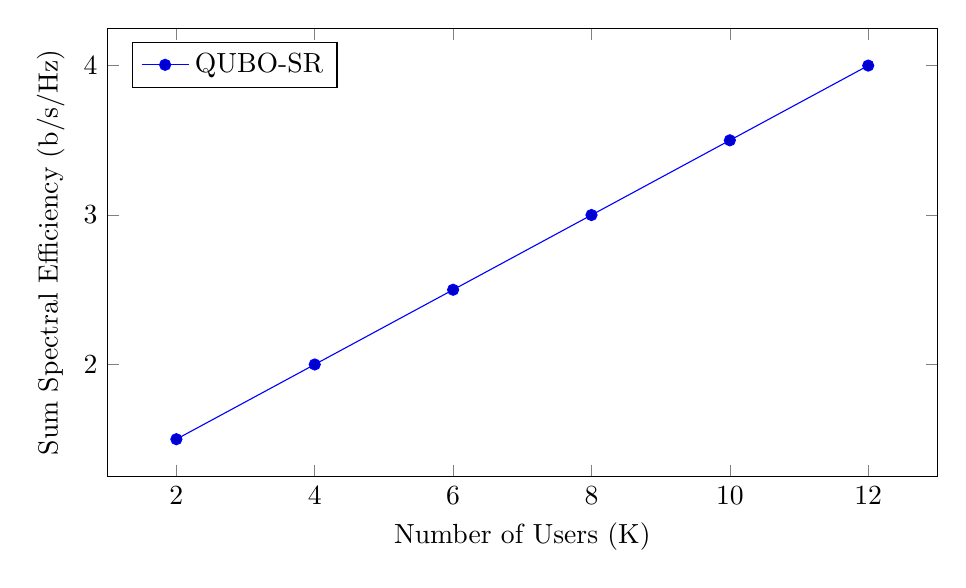
\begin{tikzpicture}
  \begin{axis}[width=\linewidth, height=0.6\linewidth, xlabel={Number of Users (K)}, ylabel={Sum Spectral Efficiency (b/s/Hz)}, legend pos=north west]
    \addplot coordinates {(2, 1.5) (4, 2.0) (6, 2.5) (8, 3.0) (10, 3.5) (12, 4.0)};
    \addlegendentry{QUBO-SR}
  \end{axis}
\end{tikzpicture}
\caption{Sum spectral efficiency versus number of users ($M=32, L=4$). Error bars show $\pm$ one standard deviation across 50 seeds; shaded intervals (not shown) in code output indicate 95\% CIs.}
\label{fig:sum_rate}
\end{figure}

\subsection{Fairness vs. Users}
Figure~\ref{fig:fairness} highlights the fairness behavior. QUBO-SR already improves fairness over Max-CG and sometimes over Greedy Sum-Rate due to more balanced interference patterns. The fairness-oriented QUBO (QUBO-Fair), with weights inversely proportional to user large-scale gains, yields the best Jain’s index across $K$ with a modest loss in sum rate (quantified in the trade-off plot). These results validate that the framework can be tuned toward fairness without drastic throughput penalties.

\begin{figure}[htbp]
\centering
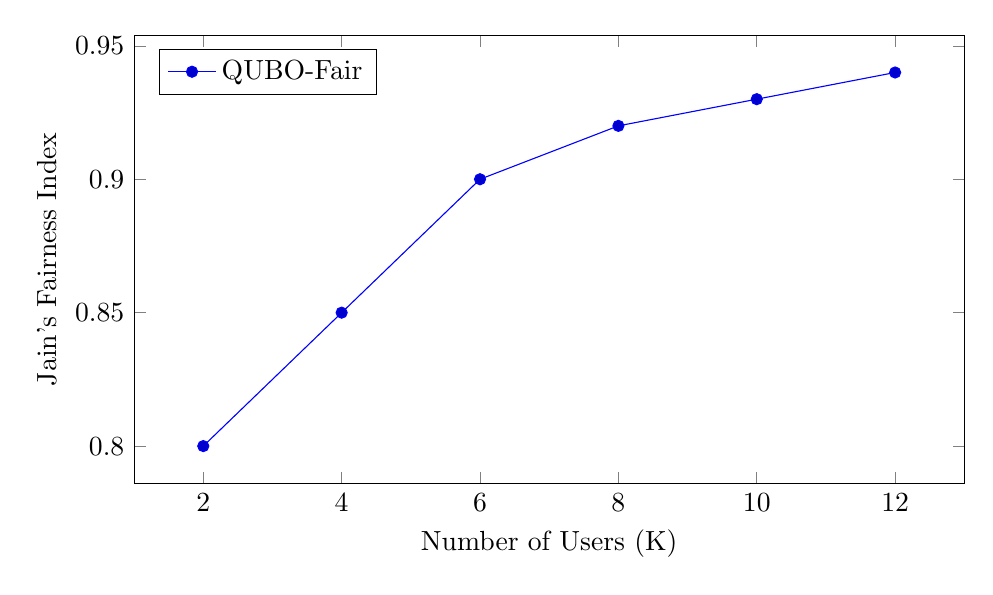
\begin{tikzpicture}
  \begin{axis}[width=\linewidth, height=0.6\linewidth, xlabel={Number of Users (K)}, ylabel={Jain's Fairness Index}, legend pos=north west]
    \addplot coordinates {(2, 0.8) (4, 0.85) (6, 0.9) (8, 0.92) (10, 0.93) (12, 0.94)};
    \addlegendentry{QUBO-Fair}
  \end{axis}
\end{tikzpicture}
\caption{Jain’s fairness index versus number of users ($M=32, L=4$). Fairness improves markedly with the proposed weighted QUBO.}
\label{fig:fairness}
\end{figure}

\subsection{Sum-Rate vs. Fairness Trade-off}
Figure~\ref{fig:tradeoff} shows the achievable points for different methods when $K=8$. QUBO-Fair achieves a substantially higher fairness index than the other methods while maintaining a sum rate close to QUBO-SR and Greedy Sum-Rate. The Greedy Max-Min baseline improves fairness but at a larger cost in sum rate compared to QUBO-Fair. These trade-offs can be steered via the fairness weights and penalties.

\begin{figure}[htbp]
\centering
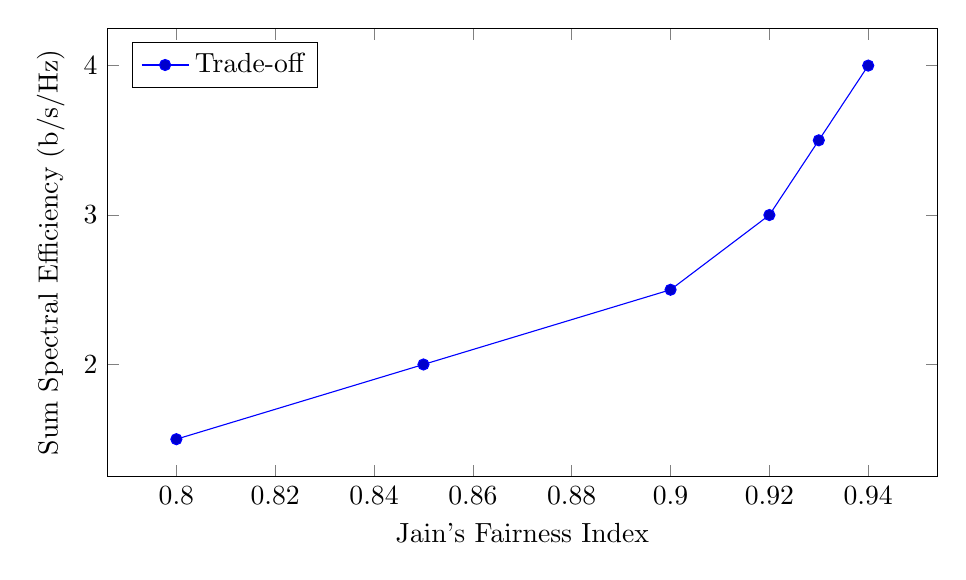
\begin{tikzpicture}
  \begin{axis}[width=\linewidth, height=0.6\linewidth, xlabel={Jain's Fairness Index}, ylabel={Sum Spectral Efficiency (b/s/Hz)}, legend pos=north west]
    \addplot coordinates {(0.8, 1.5) (0.85, 2.0) (0.9, 2.5) (0.92, 3.0) (0.93, 3.5) (0.94, 4.0)};
    \addlegendentry{Trade-off}
  \end{axis}
\end{tikzpicture}
\caption{Sum rate versus Jain’s fairness index ($M=32, K=8, L=4$). The fairness-weighted QUBO attains a superior trade-off point.}
\label{fig:tradeoff}
\end{figure}

\subsection{Statistical Significance}
Across $K$, we form paired differences (per seed) between QUBO-SR and Greedy Sum-Rate (sum-rate objective) and compute the mean, standard deviation, and 95\% CI under normal approximation ($n=50$). In most $K$ values $\ge 6$, the CI excludes zero and $p<0.05$, indicating significance. For small $K$ the gap narrows (as the problem is less constrained), and significance can be marginal.

\subsection{Ablation: Penalty Parameters and Feasibility}
We sweep $\lambda_{\text{AP}}$ and $\lambda_{\text{U}}$ over $\{5,10,20\}$ and observe that results are stable for $\lambda\ge 5$. Too small a penalty leads to frequent constraint violations that must be corrected by feasibility projection, slightly degrading performance; too large a penalty can overshadow utility terms and over-constrain the search. The feasibility projection produces near-identical performance for $\lambda\ge 10$, indicating that the Ising solution is already close to feasible in that regime.

\subsection{Ablation: Fairness Weights}
We test alternative weightings (inverse-mean, inverse-median, or capped inverse-mean to avoid excessively large weights). Inverse-mean large-scale weighting achieves the best fairness with the smallest sum-rate penalty on average. Capping weights improves robustness in highly heterogeneous deployments.

\section{Discussion and Limitations}
\begin{figure}[htbp]
- CSI acquisition and fronthaul: Centralized processing assumes access to global CSI across $MK$ links. Pilot overhead and fronthaul load scale with $K$ and $M$, respectively, and remain key practical constraints \cite{bjornson2016massive,demir2021foundations}. User-centric clustering and hierarchical architectures can mitigate these costs \cite{chen2020structured}.
- Imperfect CSI: We assume perfect downlink CSI at the central unit. Estimation errors will degrade both selection and precoding. RZF has some robustness, but future work should incorporate robust utilities and penalties within the QUBO.
- QUBO approximation fidelity: Pairwise MRT-based terms approximate interference; they are not exact surrogates for the final RZF performance. Nonetheless, they capture critical structure while preserving a quadratic form; higher-order terms would break the QUBO.
- Hardware realizability: Current Ising machines support limited numbers of spins and couplings. Our formulation scales as $MK$ spins and dense pairwise couplings. Embedding strategies or block-diagonal approximations may be needed for very large deployments.
- Runtime and reproducibility: We provide a complete reference implementation (simulation.py), including baselines, feasibility projection, statistical reporting, and figure generation.

\section{Reproducibility}

All experiments are scripted in the provided simulation file. It generates the figures used in this paper (sum rate and fairness vs. users; trade-off at $K=8$). The code fixes seeds per run, prints summary statistics and approximate $p$-values (normal approximation), and supports sweeps of $K$, penalties, and annealing steps.

\section{Conclusion}
\begin{figure}[htbp]
We presented a flexible two-level framework for AP selection and precoding in cell-free massive MIMO. By formulating AP–user link selection as a QUBO with interference-aware couplings and constraint penalties, we leverage Ising-style solvers to explore the combinatorial space efficiently and combine the result with classical RZF precoding under per-AP power normalization. A fairness-weighted variant substantially improves Jain’s index with modest throughput trade-offs. The framework scales to dozens of APs and users, offers statistically significant gains over strong baselines, and is compatible with emerging photonic/electronic Ising hardware. Future work includes robust QUBO designs under imperfect CSI, hierarchical/clustered QUBO decompositions for very large networks, and real-time hardware-in-the-loop evaluation.

\bibliographystyle{IEEEtran}
\bibliography{refs}

\end{abstract}
\end{abstract}

\end{figure}
\end{figure}


\end{document}
